\subsection*{Partie  A}
On considère la fonction $f$ définie sur $\left]-\infty ; \dfrac{3}{2}\right [$ par : \[f(x)=\dfrac{x-2}{2 x-3}\]

	\begin{enumerate}
		\item Justifier tous les éléments du tableau de variation ci-dessous.
	\end{enumerate}

	\begin{center}
	\begin{tikzpicture}
		\tkzTabInit[lgt=1,espcl=5]{$x$/1, $f$/2}{$-\infty$,$\dfrac{3}{2}$}
		\tkzTabVar{-/$\dfrac{1}{2}$,+D/$+\infty$}
	\end{tikzpicture}
	\end{center}

	\begin{enumerate}
		\setcounter{enumi}{1}
		\item En déduire que pour tout $x \in[0 ; 1]$, on a :
		\[f(x) \in[0 ; 1].\]
	\end{enumerate}

\subsection*{Partie  B}
On considère la suite $(u_{n})$ définie par :
\[\begin{cases}
	u_{0}=0 \\
	u_{n+1}=\dfrac{u_{n}-2}{2 u_{n}-3}\, ,\quad \text { pour tout entier naturel } n
\end{cases}\]

	\begin{enumerate}
		\item En utilisant la fonction $f$, démontrer par récurrence que pour tout entier naturel $n$ :
		\[0 \leqslant  u_{n} \leqslant  u_{n+1} \leqslant  1.\]

		\item En déduire que la suite $(u_{n})$ converge.

		\item On note $\ell$ la limite de la suite $(u_{n})$.

		En admettant que $\ell$ est solution de l'équation $f(x)=x$ sur l'intervalle $[0 ; 1]$, montrer que $\ell=1$.

		\item On donne ci-dessous une fonction \texttt{seuil} écrite en langage Python.

		\begin{center}
		\begin{tblr}{colspec={X[6cm,font=\ttfamily]},vlines,hline{1,Z}={solid},rowsep=0pt}
			def seuil(h):\\
			\quad n = 0\\
			\quad u = 0\\
			\quad while u < 1-h:\\
			\quad \quad n = n+1\\
			\quad \quad u = (u-2)/(2*u-3)\\
			\quad return n\\
		\end{tblr}
		\end{center}

	L'appel ~\texttt{seuil(0.0001)}~ renvoie la valeur \np{5000}.

	Interpréter cette valeur dans le contexte de l'exercice.

	\item \begin{enumerate}
		\item Donner les quatre premiers termes de la suite $\left(u_{n}\right)$ sous forme de fractions irréductibles.

		\item Conjecturer l'expression de $u_{n}$ en fonction de $n$ et démontrer cette conjecture.
	\end{enumerate}
	\end{enumerate}
